\documentclass[9pt]{article}
\usepackage[top=3cm, bottom=3cm, outer=3cm, inner=3cm]{geometry}
\usepackage{multicol}
\usepackage{graphicx}
\usepackage{url}
\usepackage{hyperref}
\usepackage{array}
\newcolumntype{x}[1]{>{\centering\arraybackslash\hspace{0pt}}p{#1}}
\usepackage{natbib}
\usepackage{multirow}
\usepackage[normalem]{ulem}
\useunder{\uline}{\ul}{}
\usepackage{listings}
\lstdefinestyle{ascii-tree}{
	literate={├}{|}1 {─}{--}1 {└}{+}1 
}
\lstset{basicstyle=\ttfamily,
	showstringspaces=false,
	commentstyle=\color{red},
	keywordstyle=\color{blue}
}
\usepackage{caption}
\usepackage{subcaption}
\usepackage{float}
\usepackage{array}
\usepackage{longtable}
\usepackage{tabularx}
\usepackage{adjustbox}
\usepackage[table]{xcolor}% http://ctan.org/pkg/xcolor
\usepackage{blindtext}
\renewcommand{\familydefault}{\sfdefault}
\usepackage{geometry}
\geometry{
	a4paper,
	total={190mm,257mm},
	left=10mm,
	top=20mm,
}
\newcolumntype{M}[1]{>{\centering\arraybackslash}m{#1}}
\newcolumntype{N}{@{}m{0pt}@{}}
%%%%%%%%%%%%%%%%%%%%%%%%%%%%%%%%%%%%%%%%%%%%%%%%%%%%%%%%%%%%%%%%%%%%%%%%%%%%
%%%%%%%%%%%%%%%%%%%%%%%%%%%%%%%%%%%%%%%%%%%%%%%%%%%%%%%%%%%%%%%%%%%%%%%%%%%%
\newcommand{\itemCourse}{Estructura de Datos y Algoritmos}
\newcommand{\itemUniversity}{Universidad Nacional de San Agustín de Arequipa}
\newcommand{\itemFaculty}{Facultad de Ingeniería de Producción y Servicios}
\newcommand{\itemDepartment}{Departamento Académico de Ingeniería de Sistemas e Informática}
\newcommand{\itemSchool}{Escuela Profesional de Ingeniería de Sistemas}
\newcommand{\itemPracticeNumber}{06}
\newcommand{\itemTheme}{Arbol AVL}
%%%%%%%%%%%%%%%%%%%%%%%%%%%%%%%%%%%%%%%%%%%%%%%%%%%%%%%%%%%%%%%%%%%%%%%%%%%%
%%%%%%%%%%%%%%%%%%%%%%%%%%%%%%%%%%%%%%%%%%%%%%%%%%%%%%%%%%%%%%%%%%%%%%%%%%%%
\usepackage[english,spanish]{babel}
\usepackage[utf8]{inputenc}
\AtBeginDocument{\selectlanguage{spanish}}
\renewcommand{\figurename}{Figura}
\renewcommand{\refname}{Referencias}
\renewcommand{\tablename}{Tabla} %esto no funciona cuando se usa babel
\AtBeginDocument{%
	\renewcommand\tablename{Tabla}
}
\usepackage{fancyhdr}
\pagestyle{fancy}
\fancyhf{}
\setlength{\headheight}{30pt}
\renewcommand{\headrulewidth}{1pt}
\renewcommand{\footrulewidth}{1pt}
\fancyhead[L]{\raisebox{-0.2\height}{
\includegraphics[width=3cm]{img/logo_episunsa.png}}}
\fancyhead[C]{\fontsize{7}{7}\selectfont	\itemUniversity \\ \itemFaculty \\ \itemDepartment \\ \itemSchool \\ \textbf{\itemCourse}}
\fancyhead[R]{\raisebox{-0.2\height}{
\includegraphics[width=1.2cm]{img/logo_abet}}}
\fancyfoot[C]{\itemCourse}
\fancyfoot[R]{Página \thepage}
\usepackage{listings}
\usepackage{color, colortbl}
\definecolor{dkgreen}{rgb}{0,0.6,0}
\definecolor{gray}{rgb}{0.5,0.5,0.5}
\definecolor{mauve}{rgb}{0.58,0,0.82}
\definecolor{codebackground}{rgb}{0.95, 0.95, 0.92}
\definecolor{tablebackground}{rgb}{0.8, 0, 0}
\lstset{frame=tb,
	language=bash,
	aboveskip=3mm,
	belowskip=3mm,
	showstringspaces=false,
	columns=flexible,
	basicstyle={\small\ttfamily},
	numbers=none,
	numberstyle=\tiny\color{gray},
	keywordstyle=\color{blue},
	commentstyle=\color{dkgreen},
	stringstyle=\color{mauve},
	breaklines=true,
	breakatwhitespace=true,
	tabsize=3,
	backgroundcolor= \color{codebackground},
}
\begin{document}
	
	\vspace*{10px}
	
	\begin{center}	
		\fontsize{17}{17} \textbf{ Informe de Laboratorio \itemPracticeNumber}
	\end{center}
	\centerline{\textbf{\Large Tema: \itemTheme}}
	%%%%%%%%%%%%%%%%%%%%%%%%%%%%%%%%%%%%%%%%%%%%%%%%%%%%%%%%%%%%%%%%%%%%%%%%%%%%
	\begin{adjustbox}{width=\textwidth}
		\begin{tabularx}{\textwidth} {
				| >{\raggedright\arraybackslash}X 
				| >{\raggedright\arraybackslash}X 
				| >{\raggedright\arraybackslash}X 
				| >{\raggedright\arraybackslash}X
				| >{\raggedright\arraybackslash}X
				| >{\raggedright\arraybackslash}X |}
			\hline
			\rowcolor{tablebackground}
			\multicolumn{6}{ | c | }{\color{white}\textbf{INFORMACIÓN BÁSICA}} \\
			\hline
			\textbf{ASIGNATURA:}& \multicolumn{5}{ | l | }{\textbf{\itemCourse}} \\
			\hline
			\textbf{TÍTULO DEL TRABAJO:} & \multicolumn{5}{ | l | }{Arbol AVL} \\
			\hline
			\textbf{NÚMERO DE TRABAJO:}& 04 & \textbf{AÑO LECTIVO:} & 2023-A & \textbf{NRO. SEMESTRE:} & III \\
			\hline
			\textbf{FECHA DE PRESENTACIÓN:} & 26/06/23 &\textbf{HORA DE PRESENTACIÓN:}& \multicolumn{3}{ | l | }{23:59} \\
			\hline
			\multicolumn{4}{ | l | }{\textbf{INTEGRANTE (s)}} & \textbf{NOTA (0-20)} & \\
			\hline
			\multicolumn{6}{ | l | }{\textbf{Hidalgo Chinchay, Paulo Andre}}\\
			\multicolumn{6}{ | l | }{\textbf{Betanzos Rosas, Taylor Anthony}}\\
			\multicolumn{6}{ | l | }{\textbf{Villafuerte Ccapira Frank Alexis}} \\
			\hline
			\multicolumn{6}{ | l | }{\textbf{DOCENTE(s):}} \\
			\multicolumn{6}{ | l | }{Mg. Edith Giovanna Cano Mamani} \\
			\hline
		\end{tabularx}
	\end{adjustbox}
	
	%%%%%%%%%%%%%%%%%%%%%%%%
	\begin{longtable}{|p{15cm}|}
		\caption{Mi tabla extendida}\\
		\hline 
		\rowcolor{tablebackground}
		\color{white}\textbf{INTRODUCCIÓN}  \\
		\hline 
		\textbf{Se implementaran los diferentes metodos con los que cuentan los AVL
		como son obtener el minimo, el maximo, buscar un elemento, eliminar un elemento,
		entre otros que seran explicados a continuacion.}  \\
		\hline 
		%%%%%%%%%%%%
		\rowcolor{tablebackground}
		\color{white}\textbf{MARCO CONCEPTUAL}  \\
		\hline 
		\textbf{Los árboles AVL son un tipo especial de árbol binario 
		de búsqueda que se caracteriza por estar balanceado. 
		Fue inventado por los matemáticos rusos Adelson-Velskii y Landis.
		 En un árbol AVL, todas las claves en su subárbol izquierdo 
		 son menores que la clave del nodo y todas las claves en el
		  subárbol derecho son mayores. La diferencia entre las alturas
		   de los subárboles de cada uno de sus nodos es, como mucho, 1}  \\
		\hline 
		%%%%%%%%%%%%
		\rowcolor{tablebackground}
		\color{white}\textbf{SOLUCIONES Y PRUEBAS}  \\
		\hline 
		\textbf{Métodos search, getMin, getMax}\\
		\textbf{Para el método search se da como argumento un nodo,
		 el cual sirve para redirigirlo a otro método search privado 
		 donde se pasan 2 nodos, con la finalidad de compararlos, 
		 se el 1er nodo que pasamos como argumento es mayor retorna
		  la búsqueda del nodo derecho, en caso no sea así, retorna
		   la búsqueda del izquierdo}\\
		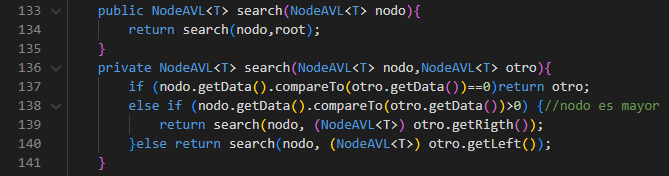
\includegraphics[width=0.85\textwidth,keepaspectratio]{img/search.png}\\
		\textbf{Para obtener el máximo solo se retorna la raíz, ya que es un AVL máximo.		}\\
		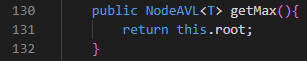
\includegraphics[width=0.6\textwidth,keepaspectratio]{img/getMax.png}\\
		\textbf{Para obtener el mínimo se usa otro método privado getMin 
		pasando como argumento un nodo, inicialmente la raíz en la cual 
		se valida que la izquierda no sea nula, en caso sea así se retorna 
		el nodo paso por argumento o si no entra recursivamente  la función 
		hasta que ya no haya más nodos a la izquierda.}  \\
		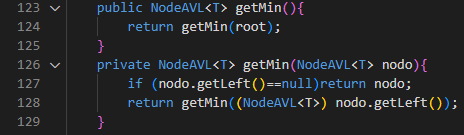
\includegraphics[width=0.8\textwidth,keepaspectratio]{img/getMin.png}\\
		
		\textbf{Para implementar la clase son aprovechamos el método search para encontrar el nodo del cual obtendremos sus nodos hijos:}  \\
		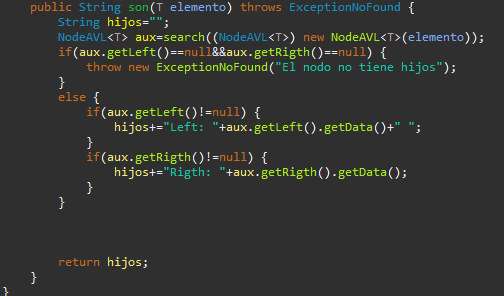
\includegraphics[width=0.8\textwidth,keepaspectratio]{img/metodoSon.png}\\
		\textbf{El metodo parent es un poco mas complicado, puesto que no podemos acceder a un nodo padre desde un nodo hijo, por lo cual será necesario buscar desde la raíz}  \\
		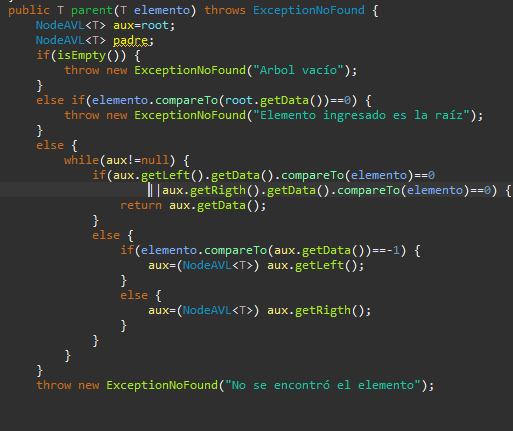
\includegraphics[width=0.8\textwidth,keepaspectratio]{img/metodoParent.png}\\
	
		\hline
		%%%%%%%%%%%%			
	\end{longtable}
	%%%%%%%%%%%%%%%%%%%%%%%%
	\begin{table}[H]
		\begin{tabular}{|p{15cm}|}
			\hline 
			\rowcolor{tablebackground}
			\color{white}\textbf{LECCIONES APRENDIDAS Y CONCLUSIONES}  \\
			\hline 
			\textbf{Se aprendio a como implementar los AVL al igual que sus metodos, co las clases auxiliares
			Node y NodeAVL, las cuales permitian tener nodos con derecha e izquierda y hallar sus resectivos
			padres e hijos.}\\
		\hline 
		%%%%%%%%%%%%
		\rowcolor{tablebackground}
		\color{white}\textbf{REFERENCIAS Y BIBLIOGRAFÍA}  \\
		\hline 
		\textbf{[]\url{https://es.wikipedia.org/wiki/Árbol_AVL}}\\
		\textbf{[]\url{https://ccia.ugr.es/~jfv/ed1/c++/cdrom5/informacion/extras/arboles_avl.pdf}}\\	
		\hline 
		%%%%%%%%%%%%			
	\end{tabular}
\end{table}
%%%%%%%%%%%%%%%%%%%%%%%%
\end{document}